% Use only LaTeX2e, calling the article.cls class and 12-point type.

\documentclass[12pt]{article}

% Users of the {thebibliography} environment or BibTeX should use the
% scicite.sty package, downloadable from *Science* at
% www.sciencemag.org/about/authors/prep/TeX_help/ .
% This package should properly format in-text
% reference calls and reference-list numbers.
\usepackage{scicite}

% Use times if you have the font installed; otherwise, comment out the
% following line.

\usepackage{times}
\usepackage{float}
\usepackage{graphicx}
\usepackage{caption}
\usepackage{subcaption}

% The preamble here sets up a lot of new/revised commands and
% environments.  It's annoying, but please do *not* try to strip these
% out into a separate .sty file (which could lead to the loss of some
% information when we convert the file to other formats).  Instead, keep
% them in the preamble of your main LaTeX source file.


% The following parameters seem to provide a reasonable page setup.

\topmargin 0.0cm
\oddsidemargin 0.2cm
\textwidth 16cm 
\textheight 21cm
\footskip 1.0cm


%The next command sets up an environment for the abstract to your paper.

\newenvironment{sciabstract}{%
\begin{quote} \bf}
{\end{quote}}


% If your reference list includes text notes as well as references,
% include the following line; otherwise, comment it out.

\renewcommand\refname{References and Notes}

% The following lines set up an environment for the last note in the
% reference list, which commonly includes acknowledgments of funding,
% help, etc.  It's intended for users of BibTeX or the {thebibliography}
% environment.  Users who are hand-coding their references at the end
% using a list environment such as {enumerate} can simply add another
% item at the end, and it will be numbered automatically.

\newcounter{lastnote}
\newenvironment{scilastnote}{%
\setcounter{lastnote}{\value{enumiv}}%
\addtocounter{lastnote}{+1}%
\begin{list}%
{\arabic{lastnote}.}
{\setlength{\leftmargin}{.22in}}
{\setlength{\labelsep}{.5em}}}
{\end{list}}
\linespread{1}

% Include your paper's title here

\title{{\bf Deep Learning Course Assignment Report}} 


% Place the author information here.  Please hand-code the contact
% information and notecalls; do *not* use \footnote commands.  Let the
% author contact information appear immediately below the author names
% as shown.  We would also prefer that you don't change the type-size
% settings shown here.

\author
{{\it Bicheng Gao,$^{1}$ Songyu Ke,$^{2}$ Yuhao Zhou$^{3}$}\\
\\
\normalsize{{\it $^{1}$volz.kz.g@gmail.com}}\\
\normalsize{{\it $^{2}$songyuke@sjtu.edu.cn}}\\
\normalsize{{\it $^{3}$yuhao\_zhou95@sjtu.edu.cn}}\\
\\
\normalsize{{\it 14 ACM class, Shanghai Jiao Tong University}}
}

% Include the date command, but leave its argument blank.

\date{}



%%%%%%%%%%%%%%%%% END OF PREAMBLE %%%%%%%%%%%%%%%%



\begin{document} 

% Double-space the manuscript.

\baselineskip24pt

% Make the title.

\maketitle 



% Place your abstract within the special {sciabstract} environment.

\begin{sciabstract}
{\bf ABSTRACT} \\
The purpose of this research is to classify the tone using the neural network and compare the differences between three neural network frameworks --- \texttt{Torch}, \texttt{MXNet} and \texttt{Theano}. Since it seems hard for the neural network to extract the feature from raw data automatically, it is necessary to preprocess the data with some proper methods. We've tried two ways of data preprocessing: eliminating the noise in all datasets or add some noise in training data to fit the environment of test data. With the processing data and Convolutional Neural Networks, we finally achieved the accuracy of {93.42\%} in \texttt{test\_new} dataset. After reaching a better performance, we keep working on comparing the frameworks and provide some major factors listing on this report.
\end{sciabstract}

% In setting up this template for *Science* papers, we've used both
% the \section* command and the \paragraph* command for topical
% divisions.  Which you use will of course depend on the type of paper
% you're writing.  Review Articles tend to have displayed headings, for
% which \section* is more appropriate; Research Articles, when they have
% formal topical divisions at all, tend to signal them with bold text
% that runs into the paragraph, for which \paragraph* is the right
% choice.  Either way, use the asterisk (*) modifier, as shown, to
% suppress numbering.

\section{Introduction}

The project of {\it Deep Learning Course} aims at constructing a proper neural network model to solve tone classification with different frameworks and discuss factors which may have an influence on the performance of each framework.\\
\\
With only the raw data, the file: \texttt{train.engy}, \  \texttt{train.f0}, \ \texttt{test.engy}, \ \texttt{test.f0},  \ \texttt{test\_new.engy}, \ \texttt{text\_new.f0}, it's a rather tough task for neural network itself to extract proper feature that may have a good performance in the test dataset. Therefore, preprocessing the data  is an appropriate way to change the data, which is much easier to train a better network. We eliminate the low energy noise and trim both heads of data. And then use cubic spline interpolation to fix the data with a proper length. However, it is not enough. We transform the data to the Mel frequency scale, divide the standard deviation of data and use an algorithm to smooth data before the interpolation.

Since the test data is recording in the noisy environment, which is totally different from the situation of training data, the other thought is to add some white noise in the training data to fit the environment of the test data. We also tried this method to evaluate the performance.

And in the {\it $2^{nd}$ Section}, we will provide all the details in our data preprocessing.
\vspace{1em}

After preprocessing the data, another major work need to be decided is the model of neural networks. With different frameworks, the implementation of each framework is different. Therefore, with the same parameters, the performance of three frameworks may have some slight changes. To choose an appropriate neural network model is complicated in many works. In this project, the total size of training data set is 400 with the fixed data shape: [$120, 1$] ([width, height]). Therefore a small model may work in a small collection of data. Fully-connected Networks and Convolutional Neural Networks are our choices, since it has excellent performance in many tasks. Meanwhile, we also try some complicated models with more layers, and the results of models comparison are also shown in the report.\\
All the information details of this part is shown in the {\it $3^{rd}$ Section} {\bf Model of Neural Networks}\\
\\
In the {\it $4^{th}$ Section} {\bf Background of the Frameworks}, we will provide the elementary information of three frameworks: \texttt{Torch}, \texttt{Theano}, \texttt{MXNet}. We will first give out a fundamental analysis of three frameworks through their own description and then compare with our own evaluations by the experiment of the tone classification in some aspects, which shown in the {\it $5^{th}$ Section} {\bf Evaluation}. We then set three major factors that may effect the implementation experience and the performance: {\bf Learning Document and Implementation Complexity}\\
\\
For the {\it $6^{th}$ Section} {\bf Future Work} Part, we're going to show some vulnerabilities of our works and the improvement that can be implemented in the future, e.g. Comparing the efficiency of GPU \& CPU, utilizing RNNs in our model, etc. And giving a {\bf conclusion} in the {\it $7^{th}$ Section}.
\\

\section{Data Preprocessing}
The following road map is the methods we've tried to deal with input data, and make the training data to fit the feature of data in \texttt{test\_new} dataset. And all the function of data\_utils are listed behind the description.
\begin{itemize}
	\item Our first version of data preprocessing is using the original data, but we use some tricks to optimize our data. The tricks are following:
		\begin{description}
			\item {\bf Ignore the low energy data.} Because when energy is low, the frequency we observe denotes the frequency of the background noise.\\
			\texttt{data\_utils.IgnoreLowEnergyFrequence(Engy, F0)}
			\item {\bf Trim the frequency data.} As we all know, the information from the frequency almost zero is not important to our learning process, so we can trim them out. 
			
				\texttt{data\_utils.TrimData(Engy, F0)}
		\end{description}
\begin{figure}[htb]
	\centering
	\begin{subfigure}[b]{0.49\textwidth}
	    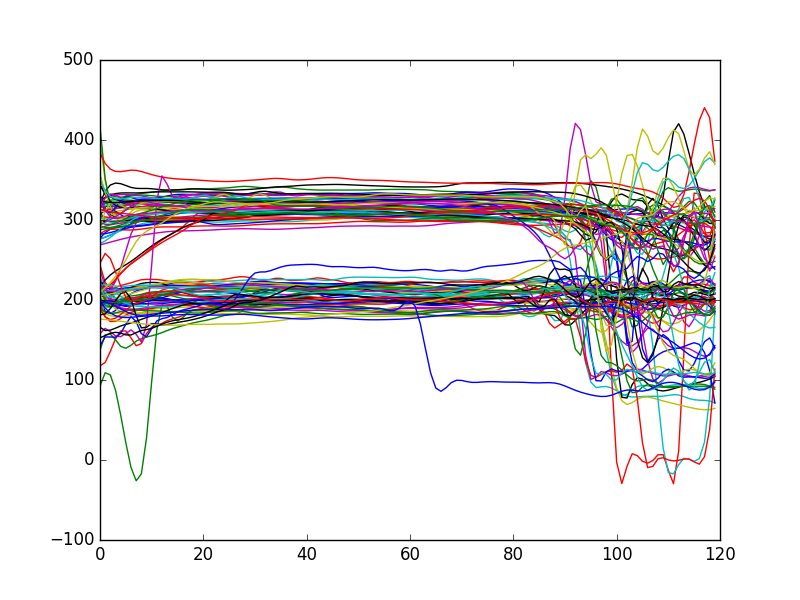
\includegraphics[width=\textwidth]{original-0}
	\end{subfigure}
	~
	\begin{subfigure}[b]{0.49\textwidth}
    	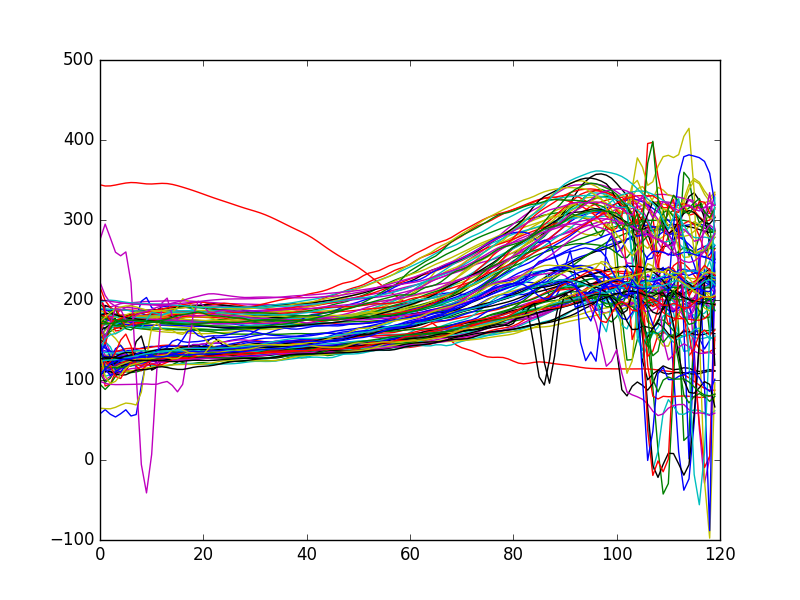
\includegraphics[width=\textwidth]{original-1}
	\end{subfigure}
	\begin{subfigure}[b]{0.49\textwidth}
	    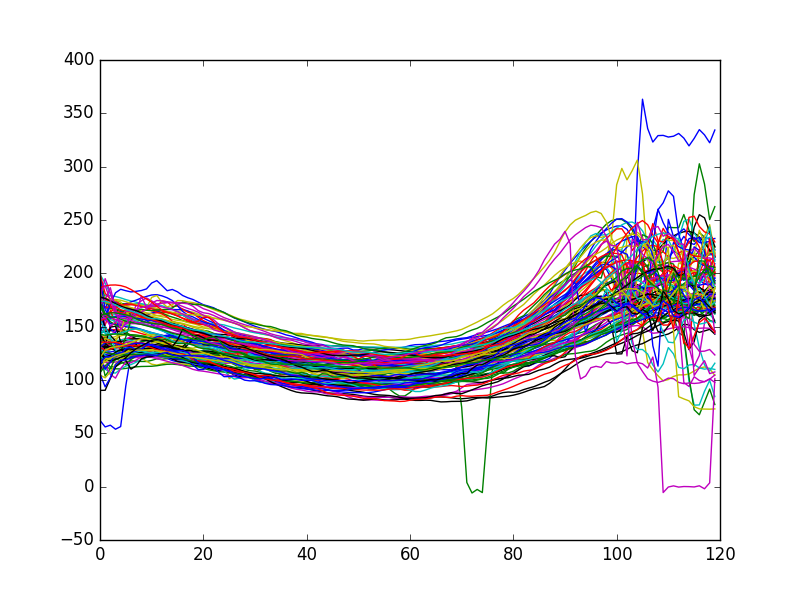
\includegraphics[width=\textwidth]{original-2}
	\end{subfigure}
	~
	\begin{subfigure}[b]{0.49\textwidth}
    	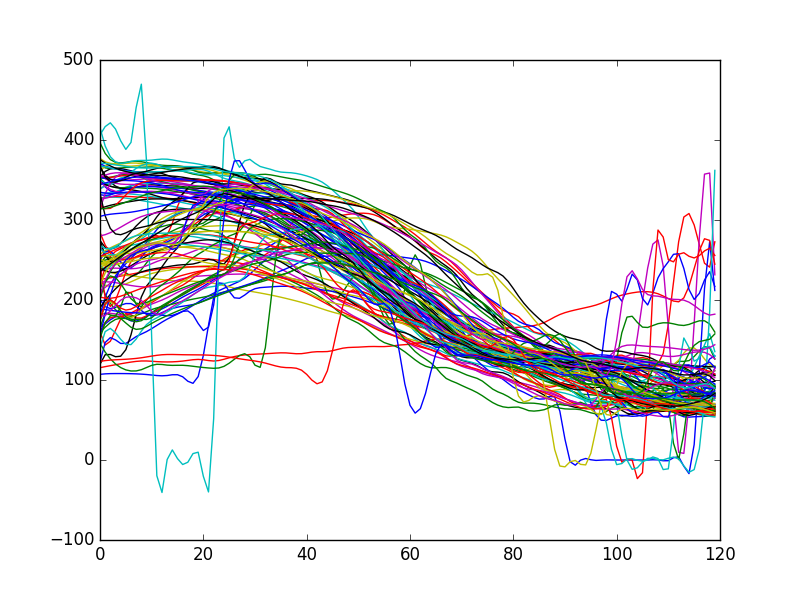
\includegraphics[width=\textwidth]{original-3}
	\end{subfigure}
	\caption{Plot of original\_data}
\end{figure}
	\item We recall the knowledge from the music class that we use octave to denote the relationship between two frequency. So we trying to take the logarithm of the data, and trying to perform our learning process in this data.
	\item Thirdly, we look up some related papers. And we found a paper named An Approach of Fundamental Frequencies Smoothing for Chinese Tone Recognition. This paper proposed an algorithm to smooth the data. There is a brief introduction:
		\begin{quote}
			The fundamental frequencies given have some obvious errors such as multiple frequency point, half frequency point and random point. The smoothing algorithm is exploited to remove them  and realize pitch curve smoothing. The algorithm proposed in the paper has several steps. Suppose $ f_1, f_2, \cdots, f_N $ are fundamental frequencies of $ N $ continuous frames. We should remove multiple frequency points and half frequency points at first. It could be done as following:

			If it has $ |f_{i} / 2 - f_{i-1}| < C_1 $ for some $ i $, then update $ f_i $ with $ f_i / 2 $. And if it has $ |f_{i} * 2 - f_{i-1}| < C_1 $ for some $ i $, then update $ f_i $ with $ f_i * 2 $.

			Then we would try to remove random error points. There are two situation:
			\begin{itemize}
				\item If $ |f_i - f_{i - 1}| > C_1 $ and $ |f_{i-1} - f_{i + 1} | > C_2 $, then we update $ f_i $ with $ 2 * f_{i - 1} - f_{i - 2} $
				\item If $ |f_i - f_{i - 1}| > C_1 $ and $ |f_{i-1} - f_{i + 1} | \leq C_2 $, then we update $ f_i $ with $ \frac{(f_{i - 1} + f_{i + 1})}{2} $.
			\end{itemize}

			By using the method above, we can get an excellent result when processing the high and level tone, the rising tone and the falling tone. But it would make some mistakes when processing the falling-rising tones. Therefore, we need to do some extra work. We can do the same work from the $ N $-th frame to the first frame.

			We take five points mean to smooth the data again at last.
		\end{quote}
	And there are steps following:
	\begin{enumerate}
		\item Transform the data to the Mel Frequency Scale.
		\item Divide the standard deviation for every data.
		\item Divide the standard deviation of full dataset for each
data.
		\item Main Smoothing method proposed by the paper.

		\texttt{data\_utils.TransformToMelFrequencyScale(F0),\\
		data\_utils.DivSingleDataStd(F0),\\
		data\_utils.DivDataStd(F0),\\
		data\_utils.SmoothF0(F0)}
		
	\end{enumerate}
\begin{figure}[htb]
	\centering
	\begin{subfigure}[b]{0.49\textwidth}
	    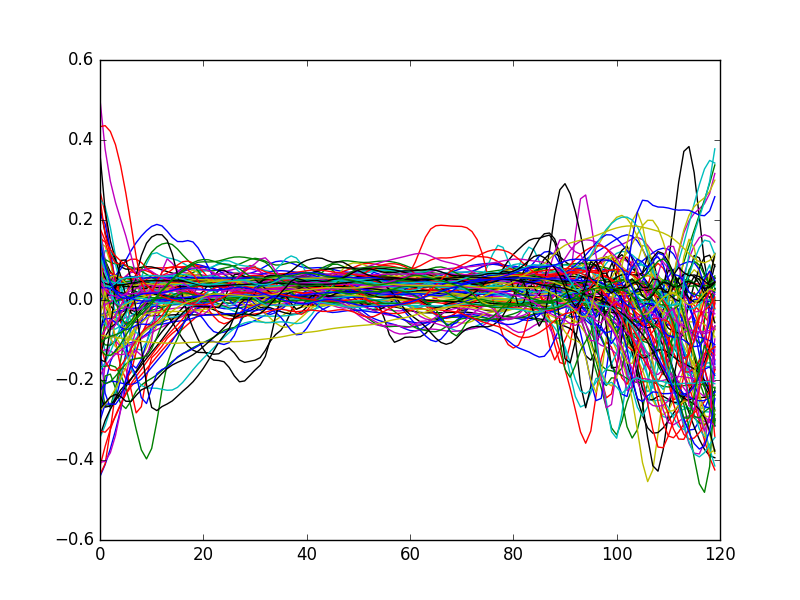
\includegraphics[width=\textwidth]{smooth-0}
	\end{subfigure}
	~
	\begin{subfigure}[b]{0.49\textwidth}
    	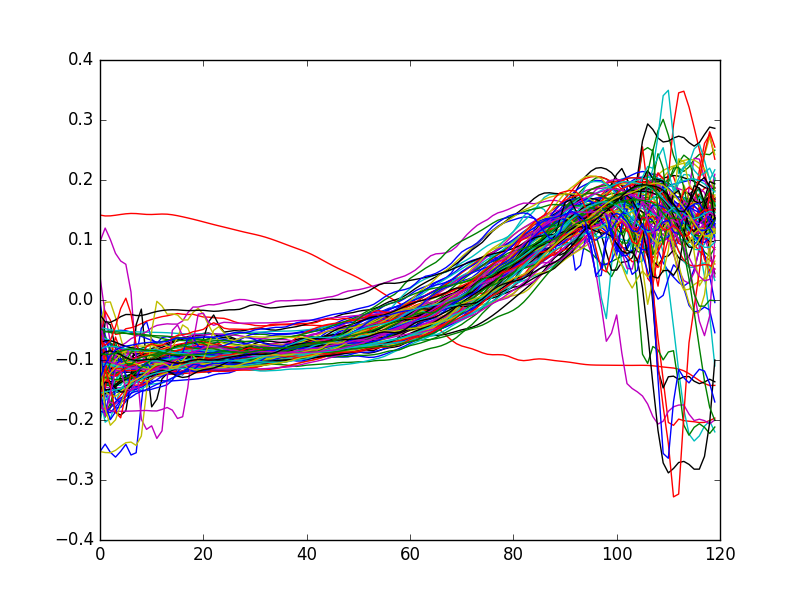
\includegraphics[width=\textwidth]{smooth-1}
	\end{subfigure}
	\begin{subfigure}[b]{0.49\textwidth}
	    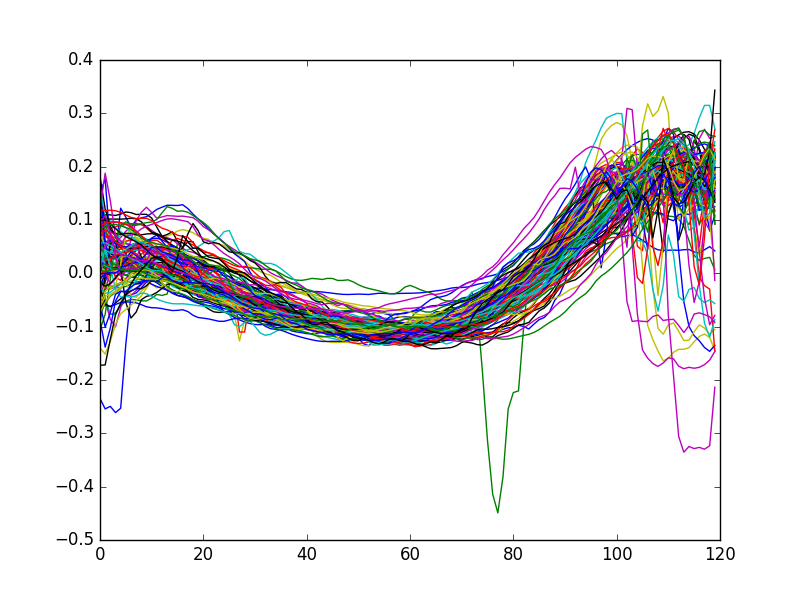
\includegraphics[width=\textwidth]{smooth-2}
	\end{subfigure}
	~
	\begin{subfigure}[b]{0.49\textwidth}
    	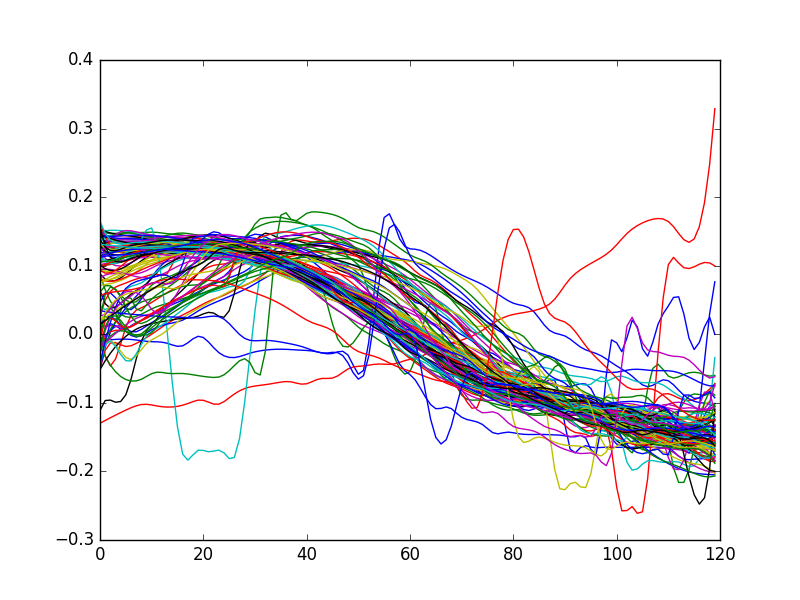
\includegraphics[width=\textwidth]{smooth-3}
	\end{subfigure}
	\caption{Plot of smooth\_data}
\end{figure}
	\item Normalization is very important in data processing, so get the mean of all data to finish the normalization. By the way, we found that we get the good result by divide the mean to finish the normalization.\\
	\texttt{data\_utils.DataSetDivideMax(F0),\\
	data\_utils.DataSetMinusMean(F0),\\
	data\_utils.NormalizeDataLengthWithInterpolation\\
	(Engy, F0, result\_len = input\_columns)}
	
	\item Next, we consider that specific environmental situation might cause the data to somehow distorted, so we trying to fit the data using quadratic function.\\
	\texttt{data\_utils.FitMissPoint(F0)}
\end{itemize}
\begin{figure}[htb]
	\centering
	\begin{subfigure}[b]{0.49\textwidth}
	    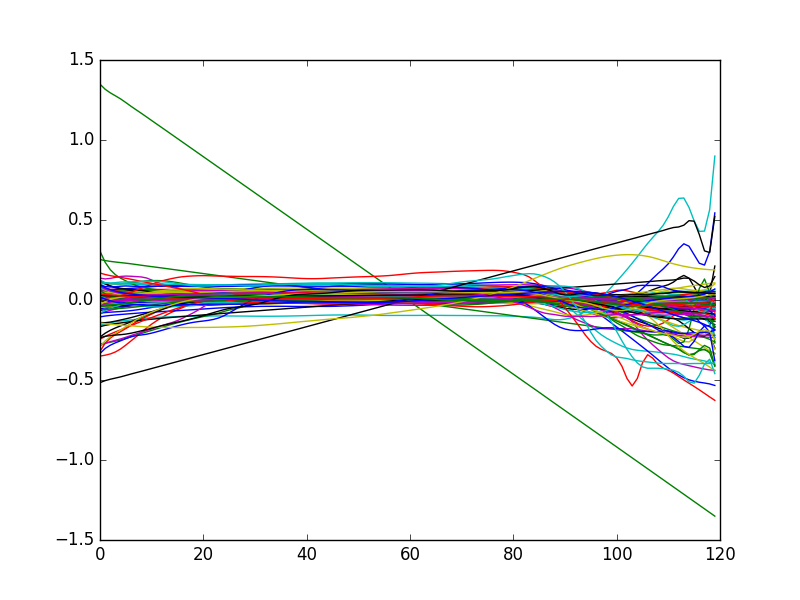
\includegraphics[width=\textwidth]{best-0}
	\end{subfigure}
	~
	\begin{subfigure}[b]{0.49\textwidth}
    	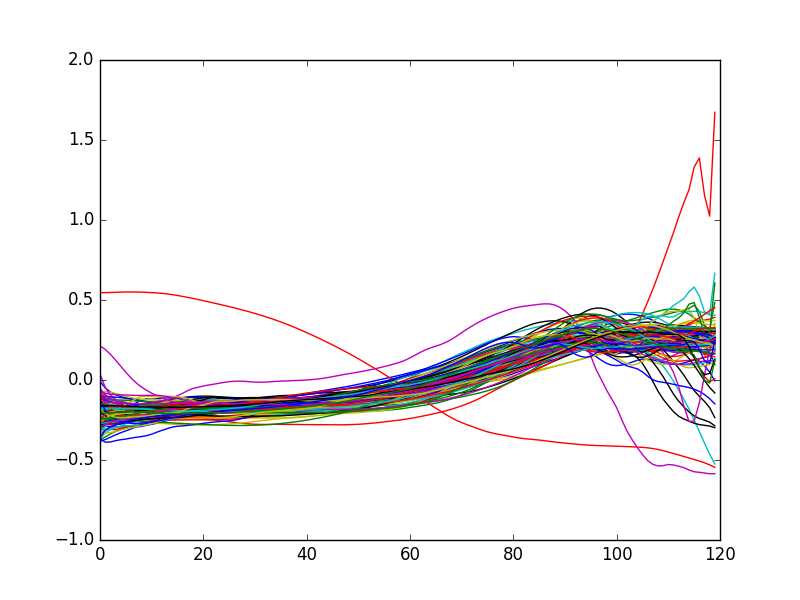
\includegraphics[width=\textwidth]{best-1}
	\end{subfigure}
	\begin{subfigure}[b]{0.49\textwidth}
	    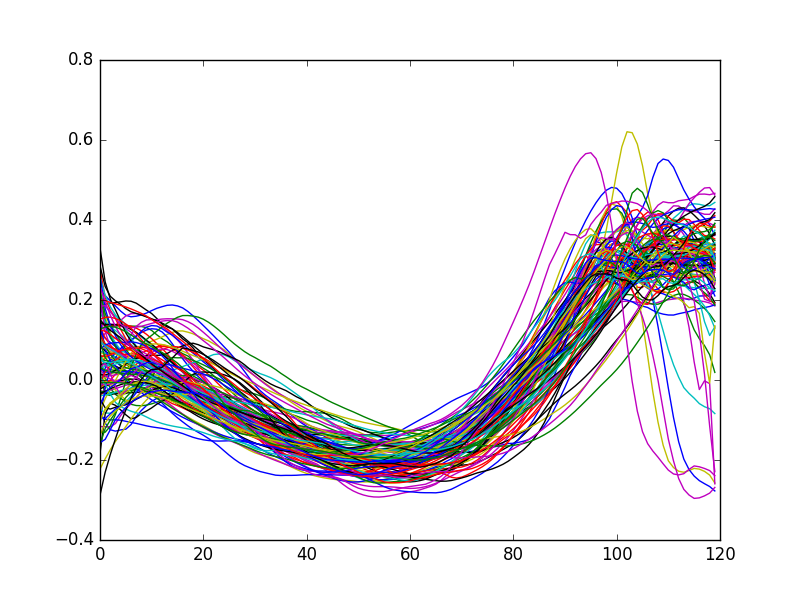
\includegraphics[width=\textwidth]{best-2}
	\end{subfigure}
	~
	\begin{subfigure}[b]{0.49\textwidth}
    	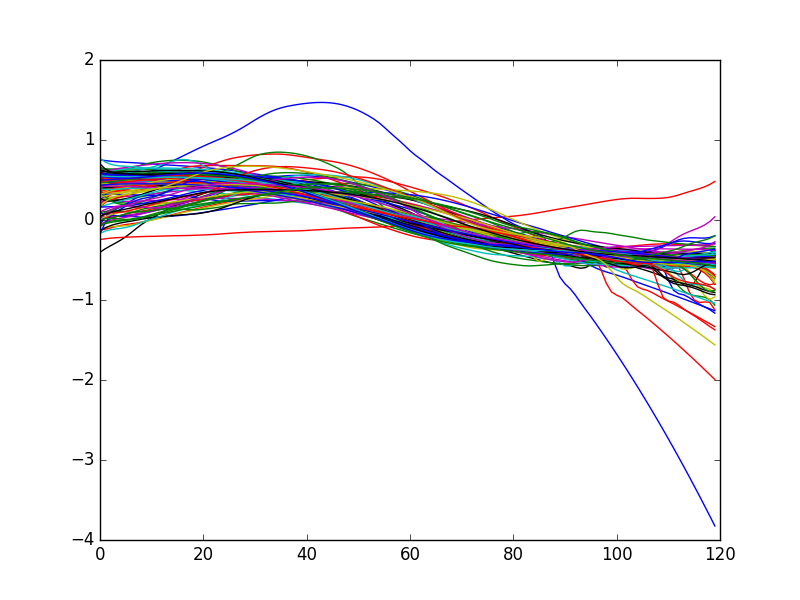
\includegraphics[width=\textwidth]{best-3}
	\end{subfigure}
	\caption{Plot of best\_data}
\end{figure}

\section{Model of Neural Networks}
In this part, we're going to show some models we used to solve tone classification. During the data processing, we've changed some parameters and models to fit the data to have a good training performance. With all models we used, the following three models can be the most representative ones for our experiment. Some may performance out of expectation, and others may have no improvement compared with simple ones. The models we shown are as follows:
\begin{itemize}
	\item {\bf Three layers of Fully Connected Networks.}
	\item {\bf Variant of the LeNet.}
	\item {\bf Variant of VGG.}
\end{itemize}

\subsection{Three layers of Fully Connected Networks}
{\it Three layers of Fully Connected Networks} is the most simple model we used, and then improve it to the Lenet to show the performance of {\it CNN layers} dealing with our data.
We first input the raw data into the {\it Three layers of Fully Connected Networks} to assure the lower bound of the test accuracy. We find that {\it Three layers of Fully Connected Networks} can also perform well with the data with only {\it ignore the low energy data} and {\it Trim the frequency data} and the accuracy can up to 80.12\%. Therefore, we've learnt from it that the net below 80\% cannot learn well with the these train dataset.

\subsection{Variant of the LeNet}

\subsection{Variant of VGG}
We also going to use a deep neural networks to show whether it is useful for the small data set to extract feature through a deep neural networks and then transfer with a net with seven {\it Convolution layers} with four {\it Pooling layers} and add two {\it Fully Connected layers} and {\it SoftmaxOutput layers}. And we will show the data performance in the {\bf Evaluation of Models}.

\subsection{Evaluation of Models}
We then evaluate all the models with our best data using \texttt{MXNet} (though it may not have the best performance, utilize its module and encapsulation, it is the simplest way to implement a networks.)
And the following table shows the models work with our best data, it shows that VGG(we've changed many parameters) is too deep to learn from the data. Also, {\it Three layers of Fully Connected Networks} performances better than the {\it LeNet}, but it might not be true for \texttt{Theano} and \texttt{Torch}

\begin{table}[!htbp]
	\caption {Model Comparison in MXNet Platform} \label{tab:title} 
	\begin{center}
		\begin{tabular}{|l|l|}
			\hline
			Model & Test-New Accuracy \\
			\hline
			3 Layer-Fully-Connected Network & 92.08\% \\
			\hline
			Variant of LeNet & 90.83\% \\
			\hline
			Variant of VGG & 20.5\% \\
			\hline
		\end{tabular}
	\end{center}
\end{table} 


\section{Background of the Frameworks}

We now keep working on the second major part of our {\it DL\_project}. Before we compare with the three models, we first list some standard information, from which we may derive inspiration of deciding the comparative factors.\\
Most of the background information are from their {\it Official Site}.

\subsection{\texttt{Torch[1]}}
The summary of core features of Torch can be listed as follows:
\begin{itemize}
	\item {\bf a powerful N-dimensional array}
	\item {\bf lots of routines for indexing, slicing, transposing, ...}
	\item {\bf amazing interface to C, via LuaJIT}
	\item {\bf linear algebra routines}
	\item {\bf neural network, and energy-based models}
	\item {\bf numeric optimization routines}
	\item {\bf Fast and efficient GPU support}
	\item {\bf Embeddable, with ports to iOS, Android and FPGA backends}
\end{itemize}
The goal of Torch is to have maximum flexibility and speed in building your scientific algorithms while making the process extremely simple. Torch comes with a large ecosystem of community-driven packages in machine learning, computer vision, signal processing, parallel processing, image, video, audio and networking among others, and builds on top of the Lua community.\\
At the heart of Torch are the popular neural network and optimization libraries which are simple to use, while having maximum flexibility in implementing complex neural network topologies. You can build arbitrary graphs of neural networks, and parallelize them over CPUs and GPUs in an efficient manner.
\subsection{\texttt{Theano[2]}}
Theano is a Python library that allows you to define, optimize, and evaluate mathematical expressions involving multi-dimensional arrays efficiently. It has some features like tight integration with NumPy, a widely used Python library in matrix process, transparent use of a GPU, efficient symbolic differentiation, speed and stability optimizations. In fact, Theano is very unfriendly for deep learning user. It has few supports to modern nenrual network. It is said that Theano is mostly used in the classroom(University of Montreal’s deep learning/machine learning classes)
\subsection{\texttt{MXNet[3]}}
MXNet is bragging as a scalable deep learning framework. It has its advantages as follows:
\begin{itemize}	
	\item {\bf Flexible Programming Model.} Supports both imperative and symbolic programming, maximizing efficiency and productivity
	\item {\bf Portable from Cloud to the Client.} Runs on CPUs or GPUs, and on clusters, servers, desktops, or mobile phones 
	\item {\bf Multiple Languages.} Supports building and training models in Python, R, Scala, Julia, and C++. Pre-trained models can be used for prediction in even more languages like Matlab or Javascript.
	\item {\bf Native Distributed Training} Supports distributed training on multiple CPU/GPU machines to take advantage of cloud scale
	\item {\bf Performance Optimized.} Parallelizes both I/O and computation with an optimized C++ backend engine, and performs optimally no matter which language you program in
\end{itemize}
And we have the following table to show a general comparison of the three frameworks.


\section{Evaluation}
In this part, we're going to give a formal evaluation system for three frameworks --- \texttt{Torch}, \texttt{Theano}, \texttt{MXNet}. With the following aspects and the general idea to these frameworks, it is rational for us to give a brief impression and further analysis to the frameworks. And the factors we use are listed as follows:
\subsection{Learning and Implementation}
\begin{itemize}
	\item  I happened to have learned this language when playing Hammperspoon in my Operating System, so it’s not a big problem for me to use the Lua as primary language. Before the implementation, I read the document of Torch platform in github. There are some examples which I can learn the global procedure of implementation. And there is a person-detection example which helps a lot in construct the overall framework for training, testing and visualization. 
	\item The tutorial on the website of Theano only teaches users how to it to do scientific computing. I search on Github to find some neural network implemented in Theano and learned how to construct and train a neural network.

	\item For MXNet, it is really a tough work for user to learning from its document. The document on the mxnet.io only list the parameters for each embedded functions and Module, and some simple description (which cannot help user to understand uses and meanings of some parameters). It should be improved, otherwise its hard to learn from the document.
		
		But for the implementation. The encapsulation and the module of MXNet might be the best implementation of all of the three frameworks. It is convenient for users to implement a linear network structures, which to some extent make up the deficiency of the document.
\end{itemize}
\subsection{Training Effect Evaluation}
We then going to evaluate the best test accuracy of each frameworks.\\
The Best Test Accuracy is achieve by different parameters in different platform, so the training time may differ in different platform when they get the best accuracy. And the data is shown in the following table.
\\
\begin{table}[!h]
	\caption {Best Accuracy for Each Platform} \label{tab:title} 
	\begin{center}
		\begin{tabular}{|l|l|l|}
			\hline
			Platform & Test Accuracy & Training Time Per Epoch\\
			\hline
			Torch & 93.42\% & 0.001027s \\
			\hline
			Theano & 90.90\% & 0.453s \\
			\hline
			MXNet & 90.83\% & 1.259s \\
			\hline
		\end{tabular}
	\end{center}
\end{table}
\\
We all use the model with two Convolution Neural Networks plus A layer of fully-connected networks and a SoftmaxOutput and with the same pooling stride and kernel as [2, 1] and with optimizer \texttt{Adam}. 
And for each frameworks, the other parameters are shown as following:\\
\centerline{param\_list = [filter\_size1, filter\_num1, filter\_size2, filter\_num2,}\\
 \centerline{num\_hidden, learning\_rate, batch\_size]}
 \centerline{param\_torch = [5, 20, 3, 50, 1000, 1e-3, 20]}
 \centerline{param\_theano = [5, 20, 3, 50, 500, 1e-5, 20]}
 \centerline{param\_mxnet = [5, 64, 3, 128, 512, 1e-5, 20]}


\begin{table}[!h]
	\caption {Performance for Different Preprocessed Dataset} \label{tab:title} 
		\begin{center}
		\begin{tabular}{|l|l|l|l|l|l|}
			\hline
			Platform & Dataset 1 & Dataset 2 & Dataset 3 & Dataset 4 & Dataset 5\\
			\hline
			Torch & 83.77\% & 27.13\% & 74.56\% & 86.4\% & 93.42\%  \\
			\hline
			Theano & 76.81\% & 72.27\% & 74.55\% &  79.55\% & 90.90\% \\
			\hline
			MXNet & 80.42\% & 71.67\% & 77.08\% & 81.67\% & 90.83\% \\
			\hline
		\end{tabular}
		\end{center}
		In table above, Dataset 1 denotes the original dataset, Dataset 2 denotes the logged Dataset 2, Dataset 3 denotes the smoothed dataset, Dataset 4 denotes the smoothed-centered dataset and Dataset 5 denotes the smoothed-centered-fitted dataset. 

\end{table} 


\subsection{Training Time Evaluation}
Since Torch is based on Lua while Theano and MXNet are based on Python, Torch runs more faster than the other two frameworks. Because our group do not have a computer with GPU, the evaluation above is based CPU.
	
\section{Future Work}
As we have spent most of dealing with the dataset, there're still many works need to be accomplished.
As for the model part, thought we've tried the several neural networks and choose {\it Three-layers Fully Connected Networks}, {\it Variant of LeNet} and {\it VGG} to represent most performance of our model, there're still many networks may work well, but we haven't tried yet.\\
Recurrent Neural Network performances well in many cases of Natural Language Processing in recent works. We guess it may also improve our model to some extent. And like Alex et al.,[4] work on Speech Recognition, RNNs may have a result out of expectation.\\
For three frameworks, there're still some problems remain to be solved. Just like MXNet, many researchers will suffer from its poor documents. Therefore, some of the effect or implementation of the embedded functions must be learnt from its open-source code. Meanwhile, MXNet has a well-performed encapsulation and module, therefore, their still many embedded functions is left to do some research. Maybe it can be another aspect for the framework evaluation.\\


\section{Conclusion}
Through this project, we know that the sometimes the model of deep learning is not the most essential part, we also need to fully exploit the potential of our dataset. If we don’t preprocess our data carefully, even if we put the most fragile model, we won’t get the satisfying result. 

And according to our group’s discussion, we also find out much difference between various frameworks. For example, the exquisite implementation of embedded optimizer may greatly increase the learning performance. And even if we take the same parameters in different frameworks, we can’t get the similar performance result. We are very excited to read the source code of open framework to figure out why they are so different. 

The following website is our project’s github repository. TAs can check it if needed. 

https://github.com/BreakVoid/DL\_Project

\section{Reference}
\noindent [1] http://torch.ch

\noindent [2] http://deeplearning.net/software/theano/

\noindent [3] http://mxnet.io/

\noindent [4] Alex Graves, Navdeep Jaitly, {\it Towards End-to-End Speech Recognition with Recurrent Neural Networks}


\end{document}




















